\subsubsection{Eliminierung 3 bis 5 Harmonischer}
Bei diesem Verfahren wurde die dritte und fünfte Harmonische eliminiert. Da es sich hierbei um einen zweiphasigen Wechselrichter handelt, ist die dritte Harmonische nicht automatisch eliminiert.\\

Um zwei Harmonische eliminieren zu können, muss das Steuersignal zwei Freiheitsgrade aufweisen.


\begin{figure}[H]
  \begin{center}
  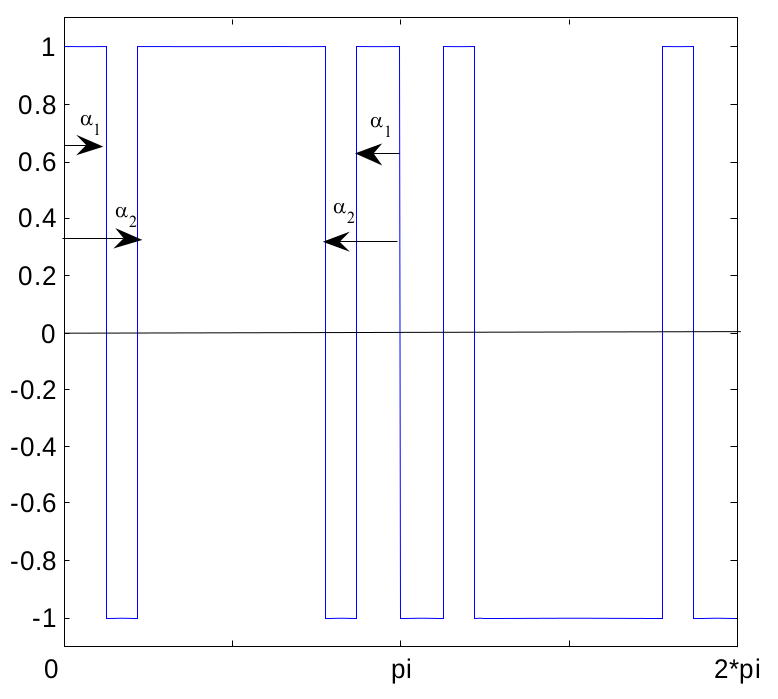
\includegraphics[width=0.48\textwidth]
  {pic/6_2_weitere_pulsmuster/6_2_1_stromform/freiheitsgrade.png}
  \caption{$Zwei Freiheitsgrade$}
  \label{fig:6_2_freiheitsgrade}
  \end{center}
\end{figure}

Durch Berechnen von $\alpha_1$ und $\alpha_2(\alpha_1)$ können bestimmte harmonische entfernt werden, in unserem Fall die dritte und fünfte.



%
% KO Pictures
%
\begin{figure}[H]
  \begin{center}
  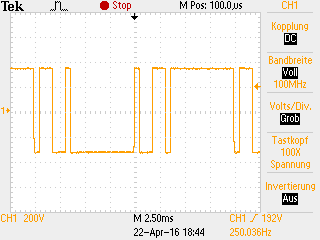
\includegraphics[width=0.48\textwidth]
  {pic/6_2_weitere_pulsmuster/6_2_1_stromform/eliminierung_3_bis_5/ALL0000/F0000TEK.png}
  \caption{$U_A (Orange)$}
  \label{fig:6_2_1_0}
  \end{center}
\end{figure}

\noindent Das Ansteuerungssignal sieht gleich aus wie in Abbilung \ref{fig:6_2_freiheitsgrade}.

\begin{figure}[H]
  \begin{center}
  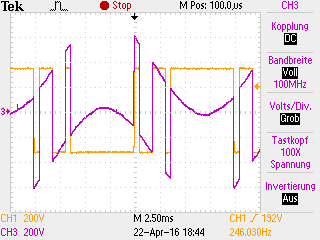
\includegraphics[width=0.48\textwidth]
  {pic/6_2_weitere_pulsmuster/6_2_1_stromform/eliminierung_3_bis_5/ALL0001/F0001TEK.png}
  \caption{$U_A (Orange), U_L (Violett)$}
  \label{fig:6_2_1_1}
  \end{center}
\end{figure}


\begin{figure}[H]
  \begin{center}
  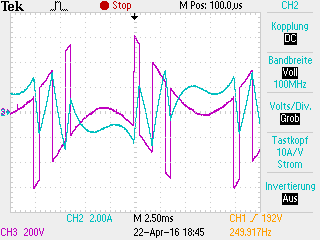
\includegraphics[width=0.48\textwidth]
  {pic/6_2_weitere_pulsmuster/6_2_1_stromform/eliminierung_3_bis_5/ALL0002/F0002TEK.png}
  \caption{$U_L (Violett), I_{L1} (Hellblau)$}
  \label{fig:6_2_1_2}
  \end{center}
\end{figure}


\clearpage